\documentclass[11pt]{article}

    \usepackage[breakable]{tcolorbox}
    \usepackage{parskip} % Stop auto-indenting (to mimic markdown behaviour)
    

    % Basic figure setup, for now with no caption control since it's done
    % automatically by Pandoc (which extracts ![](path) syntax from Markdown).
    \usepackage{graphicx}
    % Keep aspect ratio if custom image width or height is specified
    \setkeys{Gin}{keepaspectratio}
    % Maintain compatibility with old templates. Remove in nbconvert 6.0
    \let\Oldincludegraphics\includegraphics
    % Ensure that by default, figures have no caption (until we provide a
    % proper Figure object with a Caption API and a way to capture that
    % in the conversion process - todo).
    \usepackage{caption}
    \DeclareCaptionFormat{nocaption}{}
    \captionsetup{format=nocaption,aboveskip=0pt,belowskip=0pt}

    \usepackage{float}
    \floatplacement{figure}{H} % forces figures to be placed at the correct location
    \usepackage{xcolor} % Allow colors to be defined
    \usepackage{enumerate} % Needed for markdown enumerations to work
    \usepackage{geometry} % Used to adjust the document margins
    \usepackage{amsmath} % Equations
    \usepackage{amssymb} % Equations
    \usepackage{textcomp} % defines textquotesingle
    % Hack from http://tex.stackexchange.com/a/47451/13684:
    \AtBeginDocument{%
        \def\PYZsq{\textquotesingle}% Upright quotes in Pygmentized code
    }
    \usepackage{upquote} % Upright quotes for verbatim code
    \usepackage{eurosym} % defines \euro

    \usepackage{iftex}
    \ifPDFTeX
        \usepackage[T1]{fontenc}
        \IfFileExists{alphabeta.sty}{
              \usepackage{alphabeta}
          }{
              \usepackage[mathletters]{ucs}
              \usepackage[utf8x]{inputenc}
          }
    \else
        \usepackage{fontspec}
        \usepackage{unicode-math}
    \fi

    \usepackage{fancyvrb} % verbatim replacement that allows latex
    \usepackage{grffile} % extends the file name processing of package graphics
                         % to support a larger range
    \makeatletter % fix for old versions of grffile with XeLaTeX
    \@ifpackagelater{grffile}{2019/11/01}
    {
      % Do nothing on new versions
    }
    {
      \def\Gread@@xetex#1{%
        \IfFileExists{"\Gin@base".bb}%
        {\Gread@eps{\Gin@base.bb}}%
        {\Gread@@xetex@aux#1}%
      }
    }
    \makeatother
    \usepackage[Export]{adjustbox} % Used to constrain images to a maximum size
    \adjustboxset{max size={0.9\linewidth}{0.9\paperheight}}

    % The hyperref package gives us a pdf with properly built
    % internal navigation ('pdf bookmarks' for the table of contents,
    % internal cross-reference links, web links for URLs, etc.)
    \usepackage{hyperref}
    % The default LaTeX title has an obnoxious amount of whitespace. By default,
    % titling removes some of it. It also provides customization options.
    \usepackage{titling}
    \usepackage{longtable} % longtable support required by pandoc >1.10
    \usepackage{booktabs}  % table support for pandoc > 1.12.2
    \usepackage{array}     % table support for pandoc >= 2.11.3
    \usepackage{calc}      % table minipage width calculation for pandoc >= 2.11.1
    \usepackage[inline]{enumitem} % IRkernel/repr support (it uses the enumerate* environment)
    \usepackage[normalem]{ulem} % ulem is needed to support strikethroughs (\sout)
                                % normalem makes italics be italics, not underlines
    \usepackage{soul}      % strikethrough (\st) support for pandoc >= 3.0.0
    \usepackage{mathrsfs}
    

    
    % Colors for the hyperref package
    \definecolor{urlcolor}{rgb}{0,.145,.698}
    \definecolor{linkcolor}{rgb}{.71,0.21,0.01}
    \definecolor{citecolor}{rgb}{.12,.54,.11}

    % ANSI colors
    \definecolor{ansi-black}{HTML}{3E424D}
    \definecolor{ansi-black-intense}{HTML}{282C36}
    \definecolor{ansi-red}{HTML}{E75C58}
    \definecolor{ansi-red-intense}{HTML}{B22B31}
    \definecolor{ansi-green}{HTML}{00A250}
    \definecolor{ansi-green-intense}{HTML}{007427}
    \definecolor{ansi-yellow}{HTML}{DDB62B}
    \definecolor{ansi-yellow-intense}{HTML}{B27D12}
    \definecolor{ansi-blue}{HTML}{208FFB}
    \definecolor{ansi-blue-intense}{HTML}{0065CA}
    \definecolor{ansi-magenta}{HTML}{D160C4}
    \definecolor{ansi-magenta-intense}{HTML}{A03196}
    \definecolor{ansi-cyan}{HTML}{60C6C8}
    \definecolor{ansi-cyan-intense}{HTML}{258F8F}
    \definecolor{ansi-white}{HTML}{C5C1B4}
    \definecolor{ansi-white-intense}{HTML}{A1A6B2}
    \definecolor{ansi-default-inverse-fg}{HTML}{FFFFFF}
    \definecolor{ansi-default-inverse-bg}{HTML}{000000}

    % common color for the border for error outputs.
    \definecolor{outerrorbackground}{HTML}{FFDFDF}

    % commands and environments needed by pandoc snippets
    % extracted from the output of `pandoc -s`
    \providecommand{\tightlist}{%
      \setlength{\itemsep}{0pt}\setlength{\parskip}{0pt}}
    \DefineVerbatimEnvironment{Highlighting}{Verbatim}{commandchars=\\\{\}}
    % Add ',fontsize=\small' for more characters per line
    \newenvironment{Shaded}{}{}
    \newcommand{\KeywordTok}[1]{\textcolor[rgb]{0.00,0.44,0.13}{\textbf{{#1}}}}
    \newcommand{\DataTypeTok}[1]{\textcolor[rgb]{0.56,0.13,0.00}{{#1}}}
    \newcommand{\DecValTok}[1]{\textcolor[rgb]{0.25,0.63,0.44}{{#1}}}
    \newcommand{\BaseNTok}[1]{\textcolor[rgb]{0.25,0.63,0.44}{{#1}}}
    \newcommand{\FloatTok}[1]{\textcolor[rgb]{0.25,0.63,0.44}{{#1}}}
    \newcommand{\CharTok}[1]{\textcolor[rgb]{0.25,0.44,0.63}{{#1}}}
    \newcommand{\StringTok}[1]{\textcolor[rgb]{0.25,0.44,0.63}{{#1}}}
    \newcommand{\CommentTok}[1]{\textcolor[rgb]{0.38,0.63,0.69}{\textit{{#1}}}}
    \newcommand{\OtherTok}[1]{\textcolor[rgb]{0.00,0.44,0.13}{{#1}}}
    \newcommand{\AlertTok}[1]{\textcolor[rgb]{1.00,0.00,0.00}{\textbf{{#1}}}}
    \newcommand{\FunctionTok}[1]{\textcolor[rgb]{0.02,0.16,0.49}{{#1}}}
    \newcommand{\RegionMarkerTok}[1]{{#1}}
    \newcommand{\ErrorTok}[1]{\textcolor[rgb]{1.00,0.00,0.00}{\textbf{{#1}}}}
    \newcommand{\NormalTok}[1]{{#1}}

    % Additional commands for more recent versions of Pandoc
    \newcommand{\ConstantTok}[1]{\textcolor[rgb]{0.53,0.00,0.00}{{#1}}}
    \newcommand{\SpecialCharTok}[1]{\textcolor[rgb]{0.25,0.44,0.63}{{#1}}}
    \newcommand{\VerbatimStringTok}[1]{\textcolor[rgb]{0.25,0.44,0.63}{{#1}}}
    \newcommand{\SpecialStringTok}[1]{\textcolor[rgb]{0.73,0.40,0.53}{{#1}}}
    \newcommand{\ImportTok}[1]{{#1}}
    \newcommand{\DocumentationTok}[1]{\textcolor[rgb]{0.73,0.13,0.13}{\textit{{#1}}}}
    \newcommand{\AnnotationTok}[1]{\textcolor[rgb]{0.38,0.63,0.69}{\textbf{\textit{{#1}}}}}
    \newcommand{\CommentVarTok}[1]{\textcolor[rgb]{0.38,0.63,0.69}{\textbf{\textit{{#1}}}}}
    \newcommand{\VariableTok}[1]{\textcolor[rgb]{0.10,0.09,0.49}{{#1}}}
    \newcommand{\ControlFlowTok}[1]{\textcolor[rgb]{0.00,0.44,0.13}{\textbf{{#1}}}}
    \newcommand{\OperatorTok}[1]{\textcolor[rgb]{0.40,0.40,0.40}{{#1}}}
    \newcommand{\BuiltInTok}[1]{{#1}}
    \newcommand{\ExtensionTok}[1]{{#1}}
    \newcommand{\PreprocessorTok}[1]{\textcolor[rgb]{0.74,0.48,0.00}{{#1}}}
    \newcommand{\AttributeTok}[1]{\textcolor[rgb]{0.49,0.56,0.16}{{#1}}}
    \newcommand{\InformationTok}[1]{\textcolor[rgb]{0.38,0.63,0.69}{\textbf{\textit{{#1}}}}}
    \newcommand{\WarningTok}[1]{\textcolor[rgb]{0.38,0.63,0.69}{\textbf{\textit{{#1}}}}}


    % Define a nice break command that doesn't care if a line doesn't already
    % exist.
    \def\br{\hspace*{\fill} \\* }
    % Math Jax compatibility definitions
    \def\gt{>}
    \def\lt{<}
    \let\Oldtex\TeX
    \let\Oldlatex\LaTeX
    \renewcommand{\TeX}{\textrm{\Oldtex}}
    \renewcommand{\LaTeX}{\textrm{\Oldlatex}}
    % Document parameters
    % Document title
    \title{FINAL}
    
    
    
    
    
    
    
% Pygments definitions
\makeatletter
\def\PY@reset{\let\PY@it=\relax \let\PY@bf=\relax%
    \let\PY@ul=\relax \let\PY@tc=\relax%
    \let\PY@bc=\relax \let\PY@ff=\relax}
\def\PY@tok#1{\csname PY@tok@#1\endcsname}
\def\PY@toks#1+{\ifx\relax#1\empty\else%
    \PY@tok{#1}\expandafter\PY@toks\fi}
\def\PY@do#1{\PY@bc{\PY@tc{\PY@ul{%
    \PY@it{\PY@bf{\PY@ff{#1}}}}}}}
\def\PY#1#2{\PY@reset\PY@toks#1+\relax+\PY@do{#2}}

\@namedef{PY@tok@w}{\def\PY@tc##1{\textcolor[rgb]{0.73,0.73,0.73}{##1}}}
\@namedef{PY@tok@c}{\let\PY@it=\textit\def\PY@tc##1{\textcolor[rgb]{0.24,0.48,0.48}{##1}}}
\@namedef{PY@tok@cp}{\def\PY@tc##1{\textcolor[rgb]{0.61,0.40,0.00}{##1}}}
\@namedef{PY@tok@k}{\let\PY@bf=\textbf\def\PY@tc##1{\textcolor[rgb]{0.00,0.50,0.00}{##1}}}
\@namedef{PY@tok@kp}{\def\PY@tc##1{\textcolor[rgb]{0.00,0.50,0.00}{##1}}}
\@namedef{PY@tok@kt}{\def\PY@tc##1{\textcolor[rgb]{0.69,0.00,0.25}{##1}}}
\@namedef{PY@tok@o}{\def\PY@tc##1{\textcolor[rgb]{0.40,0.40,0.40}{##1}}}
\@namedef{PY@tok@ow}{\let\PY@bf=\textbf\def\PY@tc##1{\textcolor[rgb]{0.67,0.13,1.00}{##1}}}
\@namedef{PY@tok@nb}{\def\PY@tc##1{\textcolor[rgb]{0.00,0.50,0.00}{##1}}}
\@namedef{PY@tok@nf}{\def\PY@tc##1{\textcolor[rgb]{0.00,0.00,1.00}{##1}}}
\@namedef{PY@tok@nc}{\let\PY@bf=\textbf\def\PY@tc##1{\textcolor[rgb]{0.00,0.00,1.00}{##1}}}
\@namedef{PY@tok@nn}{\let\PY@bf=\textbf\def\PY@tc##1{\textcolor[rgb]{0.00,0.00,1.00}{##1}}}
\@namedef{PY@tok@ne}{\let\PY@bf=\textbf\def\PY@tc##1{\textcolor[rgb]{0.80,0.25,0.22}{##1}}}
\@namedef{PY@tok@nv}{\def\PY@tc##1{\textcolor[rgb]{0.10,0.09,0.49}{##1}}}
\@namedef{PY@tok@no}{\def\PY@tc##1{\textcolor[rgb]{0.53,0.00,0.00}{##1}}}
\@namedef{PY@tok@nl}{\def\PY@tc##1{\textcolor[rgb]{0.46,0.46,0.00}{##1}}}
\@namedef{PY@tok@ni}{\let\PY@bf=\textbf\def\PY@tc##1{\textcolor[rgb]{0.44,0.44,0.44}{##1}}}
\@namedef{PY@tok@na}{\def\PY@tc##1{\textcolor[rgb]{0.41,0.47,0.13}{##1}}}
\@namedef{PY@tok@nt}{\let\PY@bf=\textbf\def\PY@tc##1{\textcolor[rgb]{0.00,0.50,0.00}{##1}}}
\@namedef{PY@tok@nd}{\def\PY@tc##1{\textcolor[rgb]{0.67,0.13,1.00}{##1}}}
\@namedef{PY@tok@s}{\def\PY@tc##1{\textcolor[rgb]{0.73,0.13,0.13}{##1}}}
\@namedef{PY@tok@sd}{\let\PY@it=\textit\def\PY@tc##1{\textcolor[rgb]{0.73,0.13,0.13}{##1}}}
\@namedef{PY@tok@si}{\let\PY@bf=\textbf\def\PY@tc##1{\textcolor[rgb]{0.64,0.35,0.47}{##1}}}
\@namedef{PY@tok@se}{\let\PY@bf=\textbf\def\PY@tc##1{\textcolor[rgb]{0.67,0.36,0.12}{##1}}}
\@namedef{PY@tok@sr}{\def\PY@tc##1{\textcolor[rgb]{0.64,0.35,0.47}{##1}}}
\@namedef{PY@tok@ss}{\def\PY@tc##1{\textcolor[rgb]{0.10,0.09,0.49}{##1}}}
\@namedef{PY@tok@sx}{\def\PY@tc##1{\textcolor[rgb]{0.00,0.50,0.00}{##1}}}
\@namedef{PY@tok@m}{\def\PY@tc##1{\textcolor[rgb]{0.40,0.40,0.40}{##1}}}
\@namedef{PY@tok@gh}{\let\PY@bf=\textbf\def\PY@tc##1{\textcolor[rgb]{0.00,0.00,0.50}{##1}}}
\@namedef{PY@tok@gu}{\let\PY@bf=\textbf\def\PY@tc##1{\textcolor[rgb]{0.50,0.00,0.50}{##1}}}
\@namedef{PY@tok@gd}{\def\PY@tc##1{\textcolor[rgb]{0.63,0.00,0.00}{##1}}}
\@namedef{PY@tok@gi}{\def\PY@tc##1{\textcolor[rgb]{0.00,0.52,0.00}{##1}}}
\@namedef{PY@tok@gr}{\def\PY@tc##1{\textcolor[rgb]{0.89,0.00,0.00}{##1}}}
\@namedef{PY@tok@ge}{\let\PY@it=\textit}
\@namedef{PY@tok@gs}{\let\PY@bf=\textbf}
\@namedef{PY@tok@ges}{\let\PY@bf=\textbf\let\PY@it=\textit}
\@namedef{PY@tok@gp}{\let\PY@bf=\textbf\def\PY@tc##1{\textcolor[rgb]{0.00,0.00,0.50}{##1}}}
\@namedef{PY@tok@go}{\def\PY@tc##1{\textcolor[rgb]{0.44,0.44,0.44}{##1}}}
\@namedef{PY@tok@gt}{\def\PY@tc##1{\textcolor[rgb]{0.00,0.27,0.87}{##1}}}
\@namedef{PY@tok@err}{\def\PY@bc##1{{\setlength{\fboxsep}{\string -\fboxrule}\fcolorbox[rgb]{1.00,0.00,0.00}{1,1,1}{\strut ##1}}}}
\@namedef{PY@tok@kc}{\let\PY@bf=\textbf\def\PY@tc##1{\textcolor[rgb]{0.00,0.50,0.00}{##1}}}
\@namedef{PY@tok@kd}{\let\PY@bf=\textbf\def\PY@tc##1{\textcolor[rgb]{0.00,0.50,0.00}{##1}}}
\@namedef{PY@tok@kn}{\let\PY@bf=\textbf\def\PY@tc##1{\textcolor[rgb]{0.00,0.50,0.00}{##1}}}
\@namedef{PY@tok@kr}{\let\PY@bf=\textbf\def\PY@tc##1{\textcolor[rgb]{0.00,0.50,0.00}{##1}}}
\@namedef{PY@tok@bp}{\def\PY@tc##1{\textcolor[rgb]{0.00,0.50,0.00}{##1}}}
\@namedef{PY@tok@fm}{\def\PY@tc##1{\textcolor[rgb]{0.00,0.00,1.00}{##1}}}
\@namedef{PY@tok@vc}{\def\PY@tc##1{\textcolor[rgb]{0.10,0.09,0.49}{##1}}}
\@namedef{PY@tok@vg}{\def\PY@tc##1{\textcolor[rgb]{0.10,0.09,0.49}{##1}}}
\@namedef{PY@tok@vi}{\def\PY@tc##1{\textcolor[rgb]{0.10,0.09,0.49}{##1}}}
\@namedef{PY@tok@vm}{\def\PY@tc##1{\textcolor[rgb]{0.10,0.09,0.49}{##1}}}
\@namedef{PY@tok@sa}{\def\PY@tc##1{\textcolor[rgb]{0.73,0.13,0.13}{##1}}}
\@namedef{PY@tok@sb}{\def\PY@tc##1{\textcolor[rgb]{0.73,0.13,0.13}{##1}}}
\@namedef{PY@tok@sc}{\def\PY@tc##1{\textcolor[rgb]{0.73,0.13,0.13}{##1}}}
\@namedef{PY@tok@dl}{\def\PY@tc##1{\textcolor[rgb]{0.73,0.13,0.13}{##1}}}
\@namedef{PY@tok@s2}{\def\PY@tc##1{\textcolor[rgb]{0.73,0.13,0.13}{##1}}}
\@namedef{PY@tok@sh}{\def\PY@tc##1{\textcolor[rgb]{0.73,0.13,0.13}{##1}}}
\@namedef{PY@tok@s1}{\def\PY@tc##1{\textcolor[rgb]{0.73,0.13,0.13}{##1}}}
\@namedef{PY@tok@mb}{\def\PY@tc##1{\textcolor[rgb]{0.40,0.40,0.40}{##1}}}
\@namedef{PY@tok@mf}{\def\PY@tc##1{\textcolor[rgb]{0.40,0.40,0.40}{##1}}}
\@namedef{PY@tok@mh}{\def\PY@tc##1{\textcolor[rgb]{0.40,0.40,0.40}{##1}}}
\@namedef{PY@tok@mi}{\def\PY@tc##1{\textcolor[rgb]{0.40,0.40,0.40}{##1}}}
\@namedef{PY@tok@il}{\def\PY@tc##1{\textcolor[rgb]{0.40,0.40,0.40}{##1}}}
\@namedef{PY@tok@mo}{\def\PY@tc##1{\textcolor[rgb]{0.40,0.40,0.40}{##1}}}
\@namedef{PY@tok@ch}{\let\PY@it=\textit\def\PY@tc##1{\textcolor[rgb]{0.24,0.48,0.48}{##1}}}
\@namedef{PY@tok@cm}{\let\PY@it=\textit\def\PY@tc##1{\textcolor[rgb]{0.24,0.48,0.48}{##1}}}
\@namedef{PY@tok@cpf}{\let\PY@it=\textit\def\PY@tc##1{\textcolor[rgb]{0.24,0.48,0.48}{##1}}}
\@namedef{PY@tok@c1}{\let\PY@it=\textit\def\PY@tc##1{\textcolor[rgb]{0.24,0.48,0.48}{##1}}}
\@namedef{PY@tok@cs}{\let\PY@it=\textit\def\PY@tc##1{\textcolor[rgb]{0.24,0.48,0.48}{##1}}}

\def\PYZbs{\char`\\}
\def\PYZus{\char`\_}
\def\PYZob{\char`\{}
\def\PYZcb{\char`\}}
\def\PYZca{\char`\^}
\def\PYZam{\char`\&}
\def\PYZlt{\char`\<}
\def\PYZgt{\char`\>}
\def\PYZsh{\char`\#}
\def\PYZpc{\char`\%}
\def\PYZdl{\char`\$}
\def\PYZhy{\char`\-}
\def\PYZsq{\char`\'}
\def\PYZdq{\char`\"}
\def\PYZti{\char`\~}
% for compatibility with earlier versions
\def\PYZat{@}
\def\PYZlb{[}
\def\PYZrb{]}
\makeatother


    % For linebreaks inside Verbatim environment from package fancyvrb.
    \makeatletter
        \newbox\Wrappedcontinuationbox
        \newbox\Wrappedvisiblespacebox
        \newcommand*\Wrappedvisiblespace {\textcolor{red}{\textvisiblespace}}
        \newcommand*\Wrappedcontinuationsymbol {\textcolor{red}{\llap{\tiny$\m@th\hookrightarrow$}}}
        \newcommand*\Wrappedcontinuationindent {3ex }
        \newcommand*\Wrappedafterbreak {\kern\Wrappedcontinuationindent\copy\Wrappedcontinuationbox}
        % Take advantage of the already applied Pygments mark-up to insert
        % potential linebreaks for TeX processing.
        %        {, <, #, %, $, ' and ": go to next line.
        %        _, }, ^, &, >, - and ~: stay at end of broken line.
        % Use of \textquotesingle for straight quote.
        \newcommand*\Wrappedbreaksatspecials {%
            \def\PYGZus{\discretionary{\char`\_}{\Wrappedafterbreak}{\char`\_}}%
            \def\PYGZob{\discretionary{}{\Wrappedafterbreak\char`\{}{\char`\{}}%
            \def\PYGZcb{\discretionary{\char`\}}{\Wrappedafterbreak}{\char`\}}}%
            \def\PYGZca{\discretionary{\char`\^}{\Wrappedafterbreak}{\char`\^}}%
            \def\PYGZam{\discretionary{\char`\&}{\Wrappedafterbreak}{\char`\&}}%
            \def\PYGZlt{\discretionary{}{\Wrappedafterbreak\char`\<}{\char`\<}}%
            \def\PYGZgt{\discretionary{\char`\>}{\Wrappedafterbreak}{\char`\>}}%
            \def\PYGZsh{\discretionary{}{\Wrappedafterbreak\char`\#}{\char`\#}}%
            \def\PYGZpc{\discretionary{}{\Wrappedafterbreak\char`\%}{\char`\%}}%
            \def\PYGZdl{\discretionary{}{\Wrappedafterbreak\char`\$}{\char`\$}}%
            \def\PYGZhy{\discretionary{\char`\-}{\Wrappedafterbreak}{\char`\-}}%
            \def\PYGZsq{\discretionary{}{\Wrappedafterbreak\textquotesingle}{\textquotesingle}}%
            \def\PYGZdq{\discretionary{}{\Wrappedafterbreak\char`\"}{\char`\"}}%
            \def\PYGZti{\discretionary{\char`\~}{\Wrappedafterbreak}{\char`\~}}%
        }
        % Some characters . , ; ? ! / are not pygmentized.
        % This macro makes them "active" and they will insert potential linebreaks
        \newcommand*\Wrappedbreaksatpunct {%
            \lccode`\~`\.\lowercase{\def~}{\discretionary{\hbox{\char`\.}}{\Wrappedafterbreak}{\hbox{\char`\.}}}%
            \lccode`\~`\,\lowercase{\def~}{\discretionary{\hbox{\char`\,}}{\Wrappedafterbreak}{\hbox{\char`\,}}}%
            \lccode`\~`\;\lowercase{\def~}{\discretionary{\hbox{\char`\;}}{\Wrappedafterbreak}{\hbox{\char`\;}}}%
            \lccode`\~`\:\lowercase{\def~}{\discretionary{\hbox{\char`\:}}{\Wrappedafterbreak}{\hbox{\char`\:}}}%
            \lccode`\~`\?\lowercase{\def~}{\discretionary{\hbox{\char`\?}}{\Wrappedafterbreak}{\hbox{\char`\?}}}%
            \lccode`\~`\!\lowercase{\def~}{\discretionary{\hbox{\char`\!}}{\Wrappedafterbreak}{\hbox{\char`\!}}}%
            \lccode`\~`\/\lowercase{\def~}{\discretionary{\hbox{\char`\/}}{\Wrappedafterbreak}{\hbox{\char`\/}}}%
            \catcode`\.\active
            \catcode`\,\active
            \catcode`\;\active
            \catcode`\:\active
            \catcode`\?\active
            \catcode`\!\active
            \catcode`\/\active
            \lccode`\~`\~
        }
    \makeatother

    \let\OriginalVerbatim=\Verbatim
    \makeatletter
    \renewcommand{\Verbatim}[1][1]{%
        %\parskip\z@skip
        \sbox\Wrappedcontinuationbox {\Wrappedcontinuationsymbol}%
        \sbox\Wrappedvisiblespacebox {\FV@SetupFont\Wrappedvisiblespace}%
        \def\FancyVerbFormatLine ##1{\hsize\linewidth
            \vtop{\raggedright\hyphenpenalty\z@\exhyphenpenalty\z@
                \doublehyphendemerits\z@\finalhyphendemerits\z@
                \strut ##1\strut}%
        }%
        % If the linebreak is at a space, the latter will be displayed as visible
        % space at end of first line, and a continuation symbol starts next line.
        % Stretch/shrink are however usually zero for typewriter font.
        \def\FV@Space {%
            \nobreak\hskip\z@ plus\fontdimen3\font minus\fontdimen4\font
            \discretionary{\copy\Wrappedvisiblespacebox}{\Wrappedafterbreak}
            {\kern\fontdimen2\font}%
        }%

        % Allow breaks at special characters using \PYG... macros.
        \Wrappedbreaksatspecials
        % Breaks at punctuation characters . , ; ? ! and / need catcode=\active
        \OriginalVerbatim[#1,codes*=\Wrappedbreaksatpunct]%
    }
    \makeatother

    % Exact colors from NB
    \definecolor{incolor}{HTML}{303F9F}
    \definecolor{outcolor}{HTML}{D84315}
    \definecolor{cellborder}{HTML}{CFCFCF}
    \definecolor{cellbackground}{HTML}{F7F7F7}

    % prompt
    \makeatletter
    \newcommand{\boxspacing}{\kern\kvtcb@left@rule\kern\kvtcb@boxsep}
    \makeatother
    \newcommand{\prompt}[4]{
        {\ttfamily\llap{{\color{#2}[#3]:\hspace{3pt}#4}}\vspace{-\baselineskip}}
    }
    

    
    % Prevent overflowing lines due to hard-to-break entities
    \sloppy
    % Setup hyperref package
    \hypersetup{
      breaklinks=true,  % so long urls are correctly broken across lines
      colorlinks=true,
      urlcolor=urlcolor,
      linkcolor=linkcolor,
      citecolor=citecolor,
      }
    % Slightly bigger margins than the latex defaults
    
    \geometry{verbose,tmargin=1in,bmargin=1in,lmargin=1in,rmargin=1in}
    
    

\begin{document}
    
    \maketitle
    
    

    
    \section{Sketch the convolution}\label{sketch-the-convolution}

\begin{figure}
\centering
\pandocbounded{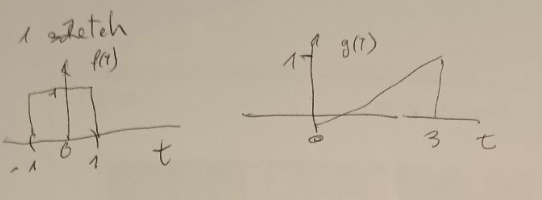
\includegraphics[keepaspectratio]{images/Fig_sketch_convo.png}}
\caption{image}
\end{figure}

{[}4 points{]}

    \begin{tcolorbox}[breakable, size=fbox, boxrule=1pt, pad at break*=1mm,colback=cellbackground, colframe=cellborder]
\prompt{In}{incolor}{1}{\boxspacing}
\begin{Verbatim}[commandchars=\\\{\}]
\PY{k}{using}\PY{+w}{ }\PY{n}{DSP}\PY{p}{,}\PY{+w}{ }\PY{n}{Plots}

\PY{c}{\PYZsh{} Define the time step for discrete convolution}
\PY{n}{dt}\PY{+w}{ }\PY{o}{=}\PY{+w}{ }\PY{l+m+mf}{0.01}
\PY{n}{t}\PY{+w}{ }\PY{o}{=}\PY{+w}{ }\PY{o}{\PYZhy{}}\PY{l+m+mi}{2}\PY{o}{:}\PY{n}{dt}\PY{o}{:}\PY{l+m+mi}{5}\PY{+w}{  }\PY{c}{\PYZsh{} Extended time range for convolution visualization}

\PY{c}{\PYZsh{} Define f(t): Rectangular Pulse from t = \PYZhy{}1 to t = 1}
\PY{n}{f}\PY{+w}{ }\PY{o}{=}\PY{+w}{ }\PY{k+kt}{Float64}\PY{p}{[}\PY{p}{(}\PY{n}{t\PYZus{}i}\PY{+w}{ }\PY{o}{\PYZgt{}=}\PY{+w}{ }\PY{o}{\PYZhy{}}\PY{l+m+mi}{1}\PY{+w}{ }\PY{o}{\PYZam{}\PYZam{}}\PY{+w}{ }\PY{n}{t\PYZus{}i}\PY{+w}{ }\PY{o}{\PYZlt{}=}\PY{+w}{ }\PY{l+m+mi}{1}\PY{p}{)}\PY{+w}{ }\PY{o}{?}\PY{+w}{ }\PY{l+m+mf}{1.0}\PY{+w}{ }\PY{o}{:}\PY{+w}{ }\PY{l+m+mf}{0.0}\PY{+w}{ }\PY{k}{for}\PY{+w}{ }\PY{n}{t\PYZus{}i}\PY{+w}{ }\PY{k}{in}\PY{+w}{ }\PY{n}{t}\PY{p}{]}

\PY{c}{\PYZsh{} Define g(t): Sawtooth function from t = 0 to t = 3 with peak at (3,1)}
\PY{n}{g}\PY{+w}{ }\PY{o}{=}\PY{+w}{ }\PY{k+kt}{Float64}\PY{p}{[}\PY{p}{(}\PY{n}{t\PYZus{}i}\PY{+w}{ }\PY{o}{\PYZgt{}=}\PY{+w}{ }\PY{l+m+mi}{0}\PY{+w}{ }\PY{o}{\PYZam{}\PYZam{}}\PY{+w}{ }\PY{n}{t\PYZus{}i}\PY{+w}{ }\PY{o}{\PYZlt{}=}\PY{+w}{ }\PY{l+m+mi}{3}\PY{p}{)}\PY{+w}{ }\PY{o}{?}\PY{+w}{ }\PY{n}{t\PYZus{}i}\PY{+w}{ }\PY{o}{/}\PY{+w}{ }\PY{l+m+mi}{3}\PY{+w}{ }\PY{o}{:}\PY{+w}{ }\PY{l+m+mf}{0.0}\PY{+w}{ }\PY{k}{for}\PY{+w}{ }\PY{n}{t\PYZus{}i}\PY{+w}{ }\PY{k}{in}\PY{+w}{ }\PY{n}{t}\PY{p}{]}

\PY{c}{\PYZsh{} Compute the convolution}
\PY{n}{y}\PY{+w}{ }\PY{o}{=}\PY{+w}{ }\PY{n}{dt}\PY{+w}{ }\PY{o}{*}\PY{+w}{ }\PY{n}{conv}\PY{p}{(}\PY{n}{f}\PY{p}{,}\PY{+w}{ }\PY{n}{g}\PY{p}{)}\PY{+w}{  }\PY{c}{\PYZsh{} Multiply by dt to approximate integral}

\PY{c}{\PYZsh{} Adjust t\PYZus{}conv to range from \PYZhy{}3 to 5}
\PY{n}{t\PYZus{}conv}\PY{+w}{ }\PY{o}{=}\PY{+w}{ }\PY{n}{range}\PY{p}{(}\PY{o}{\PYZhy{}}\PY{l+m+mi}{3}\PY{p}{,}\PY{+w}{ }\PY{n}{stop}\PY{o}{=}\PY{l+m+mi}{4}\PY{p}{,}\PY{+w}{ }\PY{n}{length}\PY{o}{=}\PY{n}{length}\PY{p}{(}\PY{n}{y}\PY{p}{)}\PY{p}{)}

\PY{c}{\PYZsh{} Plot the original signals}
\PY{n}{plot}\PY{p}{(}\PY{n}{t}\PY{p}{,}\PY{+w}{ }\PY{n}{f}\PY{p}{,}\PY{+w}{ }\PY{n}{label}\PY{o}{=}\PY{l+s}{\PYZdq{}}\PY{l+s}{f(t) (Square Pulse)}\PY{l+s}{\PYZdq{}}\PY{p}{,}\PY{+w}{ }\PY{n}{lw}\PY{o}{=}\PY{l+m+mi}{2}\PY{p}{,}\PY{+w}{ }\PY{n}{xlabel}\PY{o}{=}\PY{l+s}{\PYZdq{}}\PY{l+s}{t}\PY{l+s}{\PYZdq{}}\PY{p}{,}\PY{+w}{ }\PY{n}{ylabel}\PY{o}{=}\PY{l+s}{\PYZdq{}}\PY{l+s}{Amplitude}\PY{l+s}{\PYZdq{}}\PY{p}{,}\PY{+w}{ }\PY{n}{title}\PY{o}{=}\PY{l+s}{\PYZdq{}}\PY{l+s}{Convolution of f(t) and g(t)}\PY{l+s}{\PYZdq{}}\PY{p}{)}
\PY{n}{plot!}\PY{p}{(}\PY{n}{t}\PY{p}{,}\PY{+w}{ }\PY{n}{g}\PY{p}{,}\PY{+w}{ }\PY{n}{label}\PY{o}{=}\PY{l+s}{\PYZdq{}}\PY{l+s}{g(t) (Sawtooth Wave)}\PY{l+s}{\PYZdq{}}\PY{p}{,}\PY{+w}{ }\PY{n}{lw}\PY{o}{=}\PY{l+m+mi}{2}\PY{p}{)}

\PY{c}{\PYZsh{} Plot convolution result}
\PY{n}{plot!}\PY{p}{(}\PY{n}{t\PYZus{}conv}\PY{p}{,}\PY{+w}{ }\PY{n}{y}\PY{p}{,}\PY{+w}{ }\PY{n}{label}\PY{o}{=}\PY{l+s}{\PYZdq{}}\PY{l+s}{Convolution f * g}\PY{l+s}{\PYZdq{}}\PY{p}{,}\PY{+w}{ }\PY{n}{lw}\PY{o}{=}\PY{l+m+mi}{2}\PY{p}{,}\PY{+w}{ }\PY{n}{linestyle}\PY{o}{=}\PY{l+s+ss}{:dash}\PY{p}{)}
\end{Verbatim}
\end{tcolorbox}
 
            
\prompt{Out}{outcolor}{1}{}
    
    \begin{center}
    \adjustimage{max size={0.9\linewidth}{0.9\paperheight}}{FINAL_files/FINAL_1_0.pdf}
    \end{center}
    { \hspace*{\fill} \\}
    

    \section{\texorpdfstring{\textbf{Give the Inverse
Laplace}}{Give the Inverse Laplace}}\label{give-the-inverse-laplace}

\(H(s) = \frac{3s + 7}{s^2 - 2s - 3}\)

{[}5 points{]}

    \begin{center}\rule{0.5\linewidth}{0.5pt}\end{center}

To find the inverse Laplace transform of:

\(H(s) = \frac{3s + 7}{s^2 - 2s - 3}\)

\subsubsection{\texorpdfstring{\textbf{Step 1: Factor the
Denominator}}{Step 1: Factor the Denominator}}\label{step-1-factor-the-denominator}

Factor the quadratic denominator:

\(s^2 - 2s - 3 = (s - 3)(s + 1)\)

Thus, we rewrite:

\(H(s) = \frac{3s + 7}{(s - 3)(s + 1)}\)

\subsubsection{\texorpdfstring{\textbf{Step 2: Perform Partial Fraction
Decomposition}}{Step 2: Perform Partial Fraction Decomposition}}\label{step-2-perform-partial-fraction-decomposition}

We assume:

\(\frac{3s + 7}{(s - 3)(s + 1)} = \frac{A}{s - 3} + \frac{B}{s + 1}\)

Multiply both sides by \((s - 3)(s + 1)\) to eliminate the denominators:

\(3s + 7 = A(s + 1) + B(s - 3)\)

Expand:

\(3s + 7 = A s + A + B s - 3B\)

\(3s + 7 = (A + B)s + (A - 3B)\)

\subsubsection{\texorpdfstring{\textbf{Step 3: Solve for \(A\) and
\(B\)}}{Step 3: Solve for A and B}}\label{step-3-solve-for-a-and-b}

By comparing coefficients:

\begin{enumerate}
\def\labelenumi{\arabic{enumi}.}
\tightlist
\item
  \(A + B = 3\) (coefficient of \(s\))
\item
  \(A - 3B = 7\) (constant term)
\end{enumerate}

Solve the system:

\begin{itemize}
\tightlist
\item
  From \(A = 3 - B\), substitute into the second equation:
\end{itemize}

\(\begin{align}
(3 - B) - 3B &= 7 \\
3 - B - 3B &= 7 \\
3 - 4B &= 7 \\
-4B &= 4 \\
B &= -1
\end{align}\)

\begin{itemize}
\tightlist
\item
  Substitute \(B = -1\) into \(A = 3 - B\):
\end{itemize}

\(A = 3 - (-1) = 4\)

\subsubsection{\texorpdfstring{\textbf{Step 4: Take the Inverse Laplace
Transform}}{Step 4: Take the Inverse Laplace Transform}}\label{step-4-take-the-inverse-laplace-transform}

Now we rewrite:

\(H(s) = \frac{4}{s - 3} - \frac{1}{s + 1}\)

Using known inverse Laplace transforms:

\(\mathcal{L}^{-1} \left( \frac{1}{s - a} \right) = e^{at}\)

we get:

\(h(t) = 4e^{3t} - e^{-t}, \quad t \geq 0\)

\subsubsection{\texorpdfstring{\textbf{Final
Answer:}}{Final Answer:}}\label{final-answer}

\(h(t) = 4e^{3t} - e^{-t}, \quad t \geq 0\)

    \section{\texorpdfstring{\textbf{Causal
LTI}}{Causal LTI}}\label{causal-lti}

Input:
\(x[n] = \left(\frac{1}{2}\right)^n u[n] - \frac{1}{4} \left( \frac{1}{2}\right)^{n-1} u[n-1]\)

as output: \(y[n] = \left(\frac{1}{3}\right)^n u[n]\)

\(u[n]\) is the unit step function.

Determine: - The transfer function \(H(z)\) - The impulse response
\(h[n]\) - The corresponding difference equation

Hint: Except for the scalar, the second component of \(x[n]\) is
identical to the 1st component with a unit delay.

{[}8 points{]}

    \begin{center}\rule{0.5\linewidth}{0.5pt}\end{center}

To analyze the causal LTI system given by:

\(x[n] = \left(\frac{1}{2}\right)^n u[n] - \frac{1}{4} \left( \frac{1}{2}\right)^{n-1} u[n-1]\)

which produces the output:

\(y[n] = \left(\frac{1}{3}\right)^n u[n]\)

we will determine the transfer function \(H(z)\), the impulse response
\(h[n]\), and the difference equation.

\subsubsection{\texorpdfstring{\textbf{Step 1: Compute the Z-transform
of \(x[n]\) and
\(y[n]\)}}{Step 1: Compute the Z-transform of x{[}n{]} and y{[}n{]}}}\label{step-1-compute-the-z-transform-of-xn-and-yn}

The \textbf{Z-transform} of a geometric sequence:

\(\mathcal{Z} \left[ a^n u[n] \right] = \frac{1}{1 - a z^{-1}}, \quad |z| > |a|\)

Applying this to each term in \(x[n]\):

\begin{enumerate}
\def\labelenumi{\arabic{enumi}.}
\item
  \textbf{First term:}
  \(\mathcal{Z} \left[ \left(\frac{1}{2}\right)^n u[n] \right] = \frac{1}{1 - \frac{1}{2} z^{-1}}\)
\item
  \textbf{Second term:}
  \(\mathcal{Z} \left[ \frac{1}{4} \left( \frac{1}{2} \right)^{n-1} u[n-1] \right]\)

  \begin{itemize}
  \tightlist
  \item
    Recognizing that \(u[n-1]\) introduces a \textbf{unit delay}
    (multiplication by \(z^{-1}\) in the Z-domain):
  \end{itemize}
\end{enumerate}

\(\mathcal{Z} \left[ \left(\frac{1}{2}\right)^n u[n] \right] = \frac{1}{1 - \frac{1}{2} z^{-1}}\)

\begin{verbatim}
 So the delayed version is:
\end{verbatim}

\(z^{-1} \frac{1}{1 - \frac{1}{2} z^{-1}}\)

\begin{itemize}
\tightlist
\item
  Multiplying by \(\frac{1}{4}\):
\end{itemize}

\(\frac{1}{4} z^{-1} \frac{1}{1 - \frac{1}{2} z^{-1}}\)

Thus, the Z-transform of \(x[n]\) is:

\(X(z) = \frac{1}{1 - \frac{1}{2} z^{-1}} - \frac{1}{4} z^{-1} \frac{1}{1 - \frac{1}{2} z^{-1}}\)

Factoring:

\(X(z) = \left( 1 - \frac{1}{4} z^{-1} \right) \frac{1}{1 - \frac{1}{2} z^{-1}}\)

For \(y[n]\):

\(Y(z) = \frac{1}{1 - \frac{1}{3} z^{-1}}\)

\subsubsection{\texorpdfstring{\textbf{Step 2: Compute the Transfer
Function
\(H(z)\)}}{Step 2: Compute the Transfer Function H(z)}}\label{step-2-compute-the-transfer-function-hz}

The transfer function is:

\(H(z) = \frac{Y(z)}{X(z)}\)

\(H(z) = \frac{\frac{1}{1 - \frac{1}{3} z^{-1}}}{\left(1 - \frac{1}{4} z^{-1} \right) \frac{1}{1 - \frac{1}{2} z^{-1}}}\)

\(H(z) = \frac{(1 - \frac{1}{2} z^{-1})}{(1 - \frac{1}{4} z^{-1})(1 - \frac{1}{3} z^{-1})}\)

\subsubsection{\texorpdfstring{\textbf{Step 3: Compute the Impulse
Response
\(h[n]\)}}{Step 3: Compute the Impulse Response h{[}n{]}}}\label{step-3-compute-the-impulse-response-hn}

Since:

\(H(z) = \frac{(1 - \frac{1}{2} z^{-1})}{(1 - \frac{1}{4} z^{-1})(1 - \frac{1}{3} z^{-1})}\)

We perform \textbf{partial fraction expansion}:

\(\frac{(1 - \frac{1}{2} z^{-1})}{(1 - \frac{1}{4} z^{-1})(1 - \frac{1}{3} z^{-1})} = \frac{A}{1 - \frac{1}{4} z^{-1}} + \frac{B}{1 - \frac{1}{3} z^{-1}}\)

Multiplying by \((1 - \frac{1}{4} z^{-1})(1 - \frac{1}{3} z^{-1})\), we
get:

\(1 - \frac{1}{2} z^{-1} = A(1 - \frac{1}{3} z^{-1}) + B(1 - \frac{1}{4} z^{-1})\)

Expanding:

\(1 - \frac{1}{2} z^{-1} = A - \frac{A}{3} z^{-1} + B - \frac{B}{4} z^{-1}\)

Grouping terms:

\(( A + B ) + \left( -\frac{A}{3} - \frac{B}{4} \right) z^{-1} = 1 - \frac{1}{2} z^{-1}\)

Solving for \(A\) and \(B\):

\begin{enumerate}
\def\labelenumi{\arabic{enumi}.}
\tightlist
\item
  \(A + B = 1\)
\item
  \(-\frac{A}{3} - \frac{B}{4} = -\frac{1}{2}\)
\end{enumerate}

Solve for \(A\) and \(B\):

From \(A + B = 1\), we express \(B\) as:

\(B = 1 - A\)

Substituting into the second equation:

\(-\frac{A}{3} - \frac{(1 - A)}{4} = -\frac{1}{2}\)

Multiplying by 12 to clear fractions:

\(\begin{align*} -4A - 3 + 3A = -6 \\ -4A + 3A = -3 \\ - A = -3 \\ A = 3 \end{align*}\)

\(B = 1 - 3 = -2\)

Thus:

\(H(z) = \frac{3}{1 - \frac{1}{4} z^{-1}} - \frac{2}{1 - \frac{1}{3} z^{-1}}\)

Taking inverse Z-transform:

\(h[n] = 3 \left(\frac{1}{4}\right)^n u[n] - 2 \left(\frac{1}{3}\right)^n u[n]\)

\subsubsection{\texorpdfstring{\textbf{Step 4: Find the Difference
Equation}}{Step 4: Find the Difference Equation}}\label{step-4-find-the-difference-equation}

From:

\(Y(z) = H(z) X(z)\)

\((1 - \frac{1}{4} z^{-1})(1 - \frac{1}{3} z^{-1}) Y(z) = (1 - \frac{1}{2} z^{-1}) X(z)\)

Taking the inverse Z-transform:

\(y[n] - \frac{1}{4} y[n-1] - \frac{1}{3} y[n-1] + \frac{1}{12} y[n-2] = x[n] - \frac{1}{2} x[n-1]\)

\(y[n] - \frac{7}{12} y[n-1] + \frac{1}{12} y[n-2] = x[n] - \frac{1}{2} x[n-1]\)

\subsubsection{\texorpdfstring{\textbf{Final
Answers:}}{Final Answers:}}\label{final-answers}

\begin{enumerate}
\def\labelenumi{\arabic{enumi}.}
\item
  \textbf{Transfer Function:}
  \(\boxed{ H(z) = \frac{(1 - \frac{1}{2} z^{-1})}{(1 - \frac{1}{4} z^{-1})(1 - \frac{1}{3} z^{-1})} }\)
\item
  \textbf{Impulse Response:}
  \(\boxed{ h[n] = 3 \left(\frac{1}{4}\right)^n u[n] - 2 \left(\frac{1}{3}\right)^n u[n] }\)
\item
  \textbf{Difference Equation:}
  \(\boxed{ y[n] - \frac{7}{12} y[n-1] + \frac{1}{12} y[n-2] = x[n] - \frac{1}{2} x[n-1] }\)
\end{enumerate}

    \section{\texorpdfstring{\textbf{Continuous-time
signal}}{Continuous-time signal}}\label{continuous-time-signal}

\textbf{Continuous-time signal} contains 2 frequencies

\(x_1 = 1605 \text{ Hz}\)

\(x_2 = 1645 \text{ Hz}\)

sampled at \(10 \text{ kHz}\).

Given 200 samples, state whether or not it is possible to resolve the
two frequencies using DFT.

Discuss leakage and windowing.

{[}4 points{]}

    To determine whether it is possible to resolve the two frequencies using
the \textbf{Discrete Fourier Transform (DFT)}, we analyze the
resolution, spectral leakage, and windowing effects.

\begin{center}\rule{0.5\linewidth}{0.5pt}\end{center}

\subsubsection{\texorpdfstring{\textbf{Step 1: Frequency Resolution of
the
DFT}}{Step 1: Frequency Resolution of the DFT}}\label{step-1-frequency-resolution-of-the-dft}

The frequency resolution of a DFT is given by:

\(\Delta f = \frac{f_s}{N}\)

where: - \(f_s = 10\) kHz is the sampling frequency, - \(N = 200\) is
the number of samples.

\(\Delta f = \frac{10,000}{200} = 50 \text{ Hz}\)

The two signal frequencies are: - \(x_1 = 1605\) Hz - \(x_2 = 1645\) Hz

The frequency separation is:

\(\Delta x = 1645 - 1605 = 40 \text{ Hz}\)

Since the separation (\(40\) Hz) is \textbf{smaller} than the DFT
resolution (\(50\) Hz), \textbf{the two frequencies cannot be resolved
using a 200-point DFT}.

\begin{center}\rule{0.5\linewidth}{0.5pt}\end{center}

\subsubsection{\texorpdfstring{\textbf{Step 2: Spectral Leakage and
Windowing}}{Step 2: Spectral Leakage and Windowing}}\label{step-2-spectral-leakage-and-windowing}

\begin{itemize}
\tightlist
\item
  \textbf{Spectral leakage} occurs when a signal's frequency components
  do not align exactly with the DFT bin centers. This results in energy
  spreading across neighboring bins, making it harder to distinguish
  closely spaced frequencies.
\item
  In our case, \textbf{1605 Hz and 1645 Hz do not align with 50 Hz
  bins}, causing significant spectral leakage.
\item
  \textbf{Windowing} techniques (such as Hamming, Hanning, or Blackman)
  help reduce leakage but come at the cost of widening the main lobe in
  the frequency domain, further reducing the ability to resolve close
  frequencies.
\end{itemize}

\begin{center}\rule{0.5\linewidth}{0.5pt}\end{center}

\subsubsection{\texorpdfstring{\textbf{Conclusion}}{Conclusion}}\label{conclusion}

\begin{itemize}
\tightlist
\item
  The two frequencies \textbf{cannot be resolved} using a 200-point DFT
  due to insufficient frequency resolution (\(\Delta f = 50\) Hz
  vs.~\(\Delta x = 40\) Hz).
\item
  Spectral leakage will further blur the distinction between the two
  frequencies.
\item
  Using \textbf{zero-padding} (increasing \(N\)) or a \textbf{longer
  data record} would improve resolution.
\item
  \textbf{Applying a window function} can reduce leakage but will also
  slightly widen peaks, making resolution harder.
\end{itemize}

Thus, a \textbf{larger \(N\)} (e.g., 250 or more) is needed to reliably
separate the two frequencies.

    \section{PDF of}\label{pdf-of}

\(f(x) = A e^{- \lambda x}\)

{[}8 points{]}

    \begin{center}\rule{0.5\linewidth}{0.5pt}\end{center}

\subsubsection{probability density function
(PDF)}\label{probability-density-function-pdf}

Here is the probability density function (PDF) for the exponential
distribution:

\(f(x) = \begin{cases} A e^{-\lambda x}, & x \geq 0 \\ 0, & x < 0 \end{cases}\)

where:\\
- \(A\) is a scaling factor (often set to \(\lambda\) to ensure
normalization).\\
- \(\lambda > 0\) is the rate parameter.

If the function represents a valid probability density function, then it
must satisfy the normalization condition:

\(\int_0^\infty A e^{-\lambda x} \, dx = 1\)

Solving for \(A\):

\(A \int_0^\infty e^{-\lambda x} \, dx = 1\)

\(A \left[ \frac{e^{-\lambda x}}{-\lambda} \right]_0^\infty = 1\)

\(A \left( 0 - \left(-\frac{1}{\lambda}\right) \right) = 1\)

\(A \cdot \frac{1}{\lambda} = 1\)

\(A = \lambda\)

Thus, the standard form of the exponential distribution PDF is:

\(f(x) = \begin{cases} \lambda e^{-\lambda x}, & x \geq 0 \\ 0, & x < 0 \end{cases}\)

\subsubsection{Usage}\label{usage}

The function

\(f(x) = A e^{-\lambda x}\)

appears in various fields, particularly in \textbf{probability theory},
\textbf{physics}, \textbf{engineering}, and \textbf{signal processing}.
Here are some common contexts:

\paragraph{\texorpdfstring{\textbf{1. Probability and
Statistics}}{1. Probability and Statistics}}\label{probability-and-statistics}

\begin{itemize}
\tightlist
\item
  \textbf{Exponential Distribution}:\\
  When \(A = \lambda\) and \(x \geq 0\), this represents the probability
  density function (PDF) of an \textbf{exponential distribution}:
\end{itemize}

\(f(x) = \lambda e^{-\lambda x}, \quad x \geq 0\)

\begin{itemize}
\tightlist
\item
  Used to model \textbf{waiting times} (e.g., time between arrivals in a
  Poisson process).
\item
  Appears in \textbf{reliability analysis} (e.g., time until failure of
  a system).
\end{itemize}

\subsubsection{\texorpdfstring{\textbf{2. Engineering and Signal
Processing}}{2. Engineering and Signal Processing}}\label{engineering-and-signal-processing}

\begin{itemize}
\tightlist
\item
  \textbf{Impulse Response of an RC Circuit}:

  \begin{itemize}
  \tightlist
  \item
    The voltage or current response of a first-order low-pass filter
    follows an exponential decay.
  \end{itemize}
\item
  \textbf{Damping in Mechanical and Electrical Systems}:

  \begin{itemize}
  \tightlist
  \item
    In damped oscillatory systems, the envelope of oscillations is often
    modeled as \(A e^{-\lambda x}\).
  \end{itemize}
\item
  \textbf{Fourier and Laplace Transforms}:

  \begin{itemize}
  \tightlist
  \item
    Appears in the Laplace transform of simple decaying exponentials:
  \end{itemize}
\end{itemize}

\(\mathcal{L} \{ e^{-\lambda x} \} = \frac{1}{s + \lambda}\)

\subsubsection{\texorpdfstring{\textbf{4.
Economics}}{4. Economics}}\label{economics}

\begin{itemize}
\tightlist
\item
  \textbf{Discounted Cash Flow (DCF)}:

  \begin{itemize}
  \tightlist
  \item
    In finance, future cash flows are discounted using an exponential
    decay factor.
  \end{itemize}
\end{itemize}

\begin{center}\rule{0.5\linewidth}{0.5pt}\end{center}

\subsubsection{\texorpdfstring{\textbf{Conclusion}}{Conclusion}}\label{conclusion}

The function \(f(x) = A e^{-\lambda x}\) is widely used in modeling
\textbf{decay, probability distributions, filtering, and damping} in
multiple disciplines.

\begin{center}\rule{0.5\linewidth}{0.5pt}\end{center}

The rate parameter \(\lambda\) appears twice in the exponential
probability density function (PDF):

\(f(x) = \lambda e^{-\lambda x}, \quad x \geq 0\)

for the following reasons:

\subsubsection{\texorpdfstring{\textbf{1. Ensuring Proper
Normalization}}{1. Ensuring Proper Normalization}}\label{ensuring-proper-normalization}

A probability density function must satisfy:

\(\int_0^{\infty} f(x) \,dx = 1\)

If we assume the form \(f(x) = A e^{-\lambda x}\), we need to determine
\(A\) such that the total probability is 1:

\(\int_0^{\infty} A e^{-\lambda x} \,dx = 1\)

Using the standard integral:

\(\int_0^{\infty} e^{-\lambda x} \,dx = \frac{1}{\lambda}\)

we solve for \(A\):

\(A \cdot \frac{1}{\lambda} = 1\)

which gives \(A = \lambda\). This ensures that the total probability
sums to 1.

\subsubsection{\texorpdfstring{\textbf{2. Rate Parameter Controls Both
Scale and Decay
Rate}}{2. Rate Parameter Controls Both Scale and Decay Rate}}\label{rate-parameter-controls-both-scale-and-decay-rate}

\begin{itemize}
\tightlist
\item
  The \textbf{\(e^{-\lambda x}\)} term describes the \textbf{exponential
  decay} of probability.
\item
  The \textbf{\(\lambda\)} in front scales the function to ensure it
  integrates to 1.
\end{itemize}

Physically, \(\lambda\) represents the \textbf{average rate} of
occurrence of an event per unit time. The \textbf{mean} of an
exponentially distributed random variable is:

\(E[X] = \frac{1}{\lambda}\)

So, if \(\lambda\) is \textbf{large}, events happen frequently (fast
decay). If \(\lambda\) is \textbf{small}, events are rare (slow decay).

    \section{Linear Algebra 1}\label{linear-algebra-1}

{[}4 points{]}

    \begin{center}\rule{0.5\linewidth}{0.5pt}\end{center}

To perform curve fitting using linear algebra, follow these steps:

\begin{enumerate}
\def\labelenumi{\arabic{enumi}.}
\item
  \textbf{Choose a Model}: Select a function to fit the data (e.g.,
  linear, quadratic, exponential). Ensure the model is linear in its
  parameters (e.g., \(y = mx + b\), \(y = ax^2 + bx + c\), or linearized
  forms like \(\ln y = bx + c\) for exponentials).
\item
  \textbf{Construct the Design Matrix (A)}:

  \begin{itemize}
  \tightlist
  \item
    For a polynomial \(y = a_0 + a_1x + \dots + a_nx^n\), each row
    corresponds to a data point \((x_i, y_i)\) with entries
    \([x_i^n, x_i^{n-1}, \dots, 1]\).
  \item
    Example (linear fit for points \((1,2), (2,3), (3,5)\)):
    \(A = \begin{bmatrix} 1 & 1 \\ 2 & 1 \\ 3 & 1 \end{bmatrix}, \quad Y = \begin{bmatrix} 2 \\ 3 \\ 5 \end{bmatrix}\)
  \end{itemize}
\item
  \textbf{Formulate the Normal Equations}:

  \begin{itemize}
  \tightlist
  \item
    Compute \(A^T A\) and \(A^T Y\):
    \(A^T A = \begin{bmatrix} 14 & 6 \\ 6 & 3 \end{bmatrix}, \quad A^T Y = \begin{bmatrix} 23 \\ 10 \end{bmatrix}\)
  \item
    Solve \((A^T A) \mathbf{v} = A^T Y\) for coefficients
    \(\mathbf{v}\).
  \end{itemize}
\item
  \textbf{Solve for Coefficients}:

  \begin{itemize}
  \tightlist
  \item
    Using elimination or matrix inversion:
    \(\mathbf{v} = (A^T A)^{-1} A^T Y\)
  \item
    For the example, solving gives \(m = 1.5\), \(b = \frac{1}{3}\).
  \end{itemize}
\item
  \textbf{Verify and Use the Model}:

  \begin{itemize}
  \tightlist
  \item
    Plug coefficients into the model (e.g., \(y = 1.5x + \frac{1}{3}\)).
  \item
    Check residuals to assess fit quality.
  \end{itemize}
\end{enumerate}

\textbf{Generalization to Higher Degrees}: - For a quadratic fit,
include \(x^2\) terms in \(A\):
\(A = \begin{bmatrix} 1 & 1 & 1 \\ 4 & 2 & 1 \\ 9 & 3 & 1 \\ 16 & 4 & 1 \end{bmatrix}, \quad Y = \begin{bmatrix} 3 \\ 5 \\ 6 \\ 5 \end{bmatrix}\)
- Solve similarly to find coefficients \(a, b, c\).

\textbf{Key Considerations}: - \textbf{Numerical Stability}: Use QR
decomposition or SVD for ill-conditioned matrices. - \textbf{Nonlinear
Models}: Linearize where possible (e.g., log transforms for
exponentials).

\textbf{Final Answer}: Linear algebra facilitates curve fitting by
solving the normal equations \(A^T A \mathbf{v} = A^T Y\), yielding
coefficients that minimize the sum of squared residuals. For a best-fit
line \(y = mx + b\) through points \((1,2), (2,3), (3,5)\), the solution
is \(\boxed{y = \frac{3}{2}x + \frac{1}{3}}\).

\subsection{\texorpdfstring{relationship between \textbf{curve fitting},
\textbf{linear
algebra}}{relationship between curve fitting, linear algebra}}\label{relationship-between-curve-fitting-linear-algebra}

The relationship between \textbf{curve fitting}, \textbf{linear
algebra}, and \textbf{least squares} lies in how we approximate data
with a mathematical model by minimizing errors. Here's a breakdown:

\paragraph{\texorpdfstring{\textbf{1. Curve Fitting and Least
Squares}}{1. Curve Fitting and Least Squares}}\label{curve-fitting-and-least-squares}

\begin{itemize}
\tightlist
\item
  Curve fitting aims to find a function \(f(x)\) that best represents a
  set of data points \((x_i, y_i)\).
\item
  If the relationship is \textbf{linear in parameters}, we can express
  it as:
\end{itemize}

\(y = \beta_0 + \beta_1 x + \beta_2 x^2 + \dots + \beta_n x^n + \epsilon\)

where \(\epsilon\) is the error term. - The \textbf{least squares
method} minimizes the sum of squared errors:

\(S = \sum_{i=1}^{N} (y_i - f(x_i))^2\)

ensuring the best fit.

\paragraph{\texorpdfstring{\textbf{2. Linear Algebra
Representation}}{2. Linear Algebra Representation}}\label{linear-algebra-representation}

\begin{itemize}
\tightlist
\item
  We rewrite the problem in matrix form:
\end{itemize}

\(\mathbf{Y} = \mathbf{X} \boldsymbol{\beta} + \boldsymbol{\epsilon}\)

where: - \(\mathbf{Y}\) is the vector of observed values \(y_i\), -
\(\mathbf{X}\) is the \textbf{design matrix} containing the input data,
- \(\boldsymbol{\beta}\) is the vector of unknown parameters, -
\(\boldsymbol{\epsilon}\) is the error vector.

\begin{itemize}
\tightlist
\item
  \textbf{Example for a linear model} \(y = \beta_0 + \beta_1 x\):
\end{itemize}

\(\begin{bmatrix} y_1 \\ y_2 \\ \vdots \\ y_N \end{bmatrix} = \begin{bmatrix} 1 & x_1 \\ 1 & x_2 \\ \vdots & \vdots \\ 1 & x_N \end{bmatrix} \begin{bmatrix} \beta_0 \\ \beta_1 \end{bmatrix} + \begin{bmatrix} \epsilon_1 \\ \epsilon_2 \\ \vdots \\ \epsilon_N \end{bmatrix}\)

\paragraph{\texorpdfstring{\textbf{3. Solving for \(\boldsymbol{\beta}\)
using Least
Squares}}{3. Solving for \textbackslash boldsymbol\{\textbackslash beta\} using Least Squares}}\label{solving-for-boldsymbolbeta-using-least-squares}

\begin{itemize}
\tightlist
\item
  The least squares solution minimizes:
\end{itemize}

\(S = \| \mathbf{Y} - \mathbf{X} \boldsymbol{\beta} \|^2\)

The optimal parameters satisfy the \textbf{normal equation}:

\((\mathbf{X}^T \mathbf{X}) \boldsymbol{\beta} = \mathbf{X}^T \mathbf{Y}\)

\begin{itemize}
\tightlist
\item
  If \(\mathbf{X}^T \mathbf{X}\) is invertible, the solution is:
\end{itemize}

\(\boldsymbol{\beta} = (\mathbf{X}^T \mathbf{X})^{-1} \mathbf{X}^T \mathbf{Y}\)

\begin{itemize}
\tightlist
\item
  If not, we use \textbf{QR decomposition} or \textbf{singular value
  decomposition (SVD)}.
\end{itemize}

\paragraph{\texorpdfstring{\textbf{4. Generalization to Nonlinear
Models}}{4. Generalization to Nonlinear Models}}\label{generalization-to-nonlinear-models}

\begin{itemize}
\tightlist
\item
  Some models, like \(y = A e^{-\lambda x}\), are \textbf{nonlinear in
  parameters}.
\item
  We can linearize them (e.g., using logarithms) or use
  \textbf{nonlinear least squares} (e.g., Levenberg-Marquardt).
\end{itemize}

\paragraph{\texorpdfstring{\textbf{Summary}}{Summary}}\label{summary}

\begin{itemize}
\tightlist
\item
  \textbf{Curve fitting} finds an approximate function for given data.
\item
  \textbf{Least squares} minimizes the error between the model and data.
\item
  \textbf{Linear algebra} (matrices \& normal equations) provides an
  efficient way to solve for parameters.
\item
  \textbf{For linear models}, the solution is direct via
  \(\boldsymbol{\beta} = (\mathbf{X}^T \mathbf{X})^{-1} \mathbf{X}^T \mathbf{Y}\).
\item
  \textbf{For nonlinear models}, iterative methods like gradient descent
  or Gauss-Newton are used.
\end{itemize}

    \section{Linear Algebra 2}\label{linear-algebra-2}

{[}8 points{]}

    \(A = \begin{bmatrix} 1 & 1 & 1 & 1 \\ 2 & 1 & 4 & 3 \\ 3 & 4 & 1 & 2 \end{bmatrix}\)

Let's manually compute the \textbf{Reduced Row Echelon Form (RREF)} of
the given matrix \(A\):

\(\underbrace{\begin{bmatrix} 1 & 1 & 1 & 1 \\ 0 & -1 & 2 & 1 \\ 3 & 4 & 1 & 2 \end{bmatrix}}_{R_2 \leftarrow R_2 - 2R_1} \; \to\)
\(\underbrace{\begin{bmatrix} 1 & 1 & 1 & 1 \\ 0 & -1 & 2 & 1 \\ 0 & 1 & -2 & -1 \end{bmatrix}}_{R_3 \leftarrow R_3 - 3R_1} \; \to\)
\(\underbrace{\begin{bmatrix} 1 & 1 & 1 & 1 \\ 0 & 1 & -2 & -1 \\ 0 & 1 & -2 & -1 \end{bmatrix}}_{R_2 \leftarrow -R_2} \; \to\)
\(\underbrace{\begin{bmatrix} 1 & 1 & 1 & 1 \\ 0 & 1 & -2 & -1 \\ 0 & 0 & 0 & 0 \end{bmatrix}}_{R_3 \leftarrow R_3 - R_2} \; \to\)
\(\underbrace{\begin{bmatrix} 1 & 0 & 3 & 2 \\ 0 & 1 & -2 & -1 \\ 0 & 0 & 0 & 0 \end{bmatrix}}_{R_1 \leftarrow R_1 - R_2}\)

\subsubsection{\texorpdfstring{\textbf{Final RREF:} (Reduced Row Echelon
Form)}{Final RREF: (Reduced Row Echelon Form)}}\label{final-rref-reduced-row-echelon-form}

\(\begin{bmatrix} \underbrace{1}_{\text{pivot}} & 0 & 3 & 2 \\ 0 & \underbrace{1}_{\text{pivot}} & -2 & -1 \\ 0 & 0 & 0 & 0 \end{bmatrix}\)
\(\begin{bmatrix}
   x_1 \\
   x_2 \\
   x_3 \\
   x_4
\end{bmatrix} =
\begin{bmatrix}
   0 \\
   0 \\
   0
\end{bmatrix}\)

\(C(A) = \text{ column span of A }\left( \begin{bmatrix}
                       1 \\
                       2 \\
                       3
                    \end{bmatrix}
                    \begin{bmatrix}
                       1 \\
                       1 \\
                       4
                    \end{bmatrix}
                    \begin{bmatrix}
                       1 \\
                       4 \\
                       1
                    \end{bmatrix}
                    \begin{bmatrix}
                       1 \\
                       3 \\
                       2
                    \end{bmatrix}
                \right)\)

The Null Space \(N(A) = N( rref(A) )\) is a set of all vectors that
satisfy :

\(\begin{align}
x_1 + 0 x_2 + 3 x_3 + 2 x_4 = 0 \\
0 x_1 + x_2 - \underbrace{2 x_3}_{x_3\text{ free}} -   \underbrace{x_4}_{x_4\text{ free}} = 0
\end{align}\)

let's solve the pivot entries

\(\begin{align}
x_1 &= - 3 x_3 - 2 x_4 \\
x_2 &= 2 x_3 + x_4
\end{align}\)

\(\text{Col}_3 = 3 \begin{bmatrix}
       1 \\
       2 \\
       3
    \end{bmatrix} + (-2)
    \begin{bmatrix}
       1 \\
       1 \\
       4
    \end{bmatrix}\)
\(\text{Col}_4 = 2 \cdot \text{Col}_1 + (-1) \cdot \text{Col}_2\)

\(\left\{ \begin{bmatrix}
       1 \\
       2 \\
       3
    \end{bmatrix}
    \begin{bmatrix}
       1 \\
       1 \\
       4
    \end{bmatrix}
\right\} \text{ is the basis for C(A) }\)

    \begin{itemize}
\tightlist
\item
  \href{https://www.youtube.com/watch?v=_uTAdf_AsfQ}{Null space and
  column space basis \textbar{} Vectors and spaces \textbar{} Linear
  Algebra \textbar{} Khan Academy}
\end{itemize}


    % Add a bibliography block to the postdoc
    
    
    
\end{document}
